Nous allons maintenant étudier un des outils les plus évolués en matière de fact-checking automatique. Cette étude va nous permettre de mettre en lumière les enjeux et challenges pour aboutir à un système autonome.

\paragraph{Claimbuster} \cite{hassan2017claimbuster} \cite{hassan2015quest}

ClaimnBuster est ce qu'on appel un Fact checking system, c'est-à-dire un un système qui va procéder de manière automatique, du moins en partie, à une ou plusieurs étapes de vérification d'un fait. Ce système permet d'extraire des faits d'une source de données et de leur appliquer un score qui détermine si un fait est plus ou moins vérifiable. ClaimBuster est utilisé pour faciliter le processus de vérification de fait, il a pour fonction d'aider le journaliste dans son travail. Cet outil va permettre au journaliste de se concentrer sur la vérification d'un fait plutôt que sur son identification et son extraction. Claimbuster est spécialisé dans la vérification de faits liés à la sphère politique.
\\*
Il se construit autour de différentes techniques d'apprentissage et de traitement de données : l'apprentissage automatique (machine learning), le traitement automatique du langage naturel, etc.
Il est aussi capable, sur certains faits, d'appliquer automatiquement un état qui défini si un fait est plus ou moins vrai. Dans certains cas, ce système est entièrement autonome. Pour ce type de scénario, ClaimBuster dispose de 2 méthodes pour vérifier un fait. 

Soit il va questionner des sources de données de faits déjà vérifiés et dans ce cas il ne se présente que comme une interface entre le fait et sa vérification. Dans le second cas il est capable de produire un verdict en traduisant le fait en question. Il requête ensuite des systèmes de type question-réponses (exemple : Google), compare et confronte les résultats pour établir son verdict.

\begin{figure}[ht]
\centering
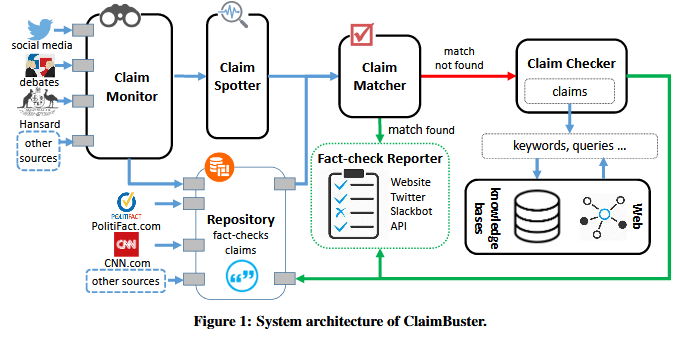
\includegraphics[width=\textwidth, draft=false]{imgs/claimbuster.PNG}
\caption{Architecture de ClaimBuster}
\label{claimbuster}
\end{figure}

\paragraph{ClaimMonitor}

C'est le module qui recherche et récupère les données. Au travers de différentes sources de données il va rechercher des textes à analyser. Ce module travaille sur 3 différentes sources de données. Il y a tout d'abord la nécessité de travailler sur des informations en live afin de pouvoir instantanément évaluer les propos d'une personne : les débats politiques par exemple. C'est pour cela que les médias audiovisuels sont une importante source de données. ClaimBuster utilise différentes api pour traduire ce flux en données utilisables, notamment la structuration des données au travers de l'identification de l'orateur \cite{joseph2015speaker}. Ensuite le Claim Monitor travaille sur les données disponibles via les réseaux sociaux, il suit 2220 compte Twitter appartenant à différents type d'entité (personnalité politique, médias d'information, etc.). Seul les tweets relatifs à la politique sont gardés. Enfin ce module récupère diverses information issues de plusieurs sites web.

\paragraph{ClaimSpotter}

Une fois l'information captée et filtrée, on se retrouve avec des données liées à la politique et potentiellement constatables. Actuellement l'élément de ClaimBuster le plus mature est le Claim Spotter qui va attribuer un score à une assertion en fonction de si le fait définit est plus ou moins vérifiable : proche de 1, le fait peut être vérifié, proche de 0 le fait n'est pas vérifiable. Ce module a été construit autour d'un modèle définit par plusieurs dizaines de milliers de fait vérifiés manuellement. La précision de ce modèle est de plus de 80\%.  Le processus peut éventuellement s'arrêter à cette étape si les prochaines étapes n'apportent pas d'informations concluantes. Dans ce cas on va simplement retourner à l'utilisateur une suite de faits définis comme vérifiables et leurs scores.

Le ClaimSpotter et l'identification des faits potentiellement vérifiable s'est fait au travers du machine learning et l'apprentissage supervisé (ici on travail sur des données vérifiées). Le set de données est composé de plusieurs dizaines de milliers de phrases prononcées durant des discours, débats, etc. politiques. Chaque phrase est identifiée comme étant plus ou moins importante et plus ou moins vérifiable. PLus précisément on différencie les : 
\begin{itemize}
    \item NFS (Non Factual Sense) : qui sont des phrases banales décrivant des opinions, des traits d'humour, etc. 
    \item UFS (Unimportant Factual Sentence) : représente des phrase qui décrivent des faits qui n'ont que peu d'importance, ex : "Demain il va pleuvoir"
    \item CFS (Check-worthy Factual Sentence) : des phrases digne d'intérêts, qui valent la peine d'être vérifiées. 
\end{itemize}

Afin de noter et classifier ces phrases, ClaimBuster va utiliser des Support Vector Machines (SVM), en français, séparateurs à vaste marge. Les SVM sont une classe d'algorithmes d'apprentissage supervisée destinés à la prévision de variable qualitative binaire, c'est-à-dire des problèmes de discrimination. Plus précisément, si l'on prend une phrase de type CFS, on va la traiter comme étant positive (les autres types étant négatifs). La SVM va ensuite trouver la marge optimale et tenter de trouver un classifieur permettant de généraliser et séparer les observations et ainsi leur attribuer un score distinctif.

\paragraph{ClaimMatcher}

A partir de cette étape, on ne travail que sur des faits définis comme vérifiables, on a éliminé les opinions et tout ce qui n'est pas une assertion. Ainsi étant donné une phrase qui énonce un fait, on va essayer de prouver ou non sa véracité. Le ClaimMatcher va tenter de trouver des faits déjà vérifiés (issus de plusieurs site de fack-checking) et en rapport avec l'assertion. Pour cela il utilise 2 méthodes, l'une consiste à simplement établir une concordance entre les mots utilisés pour qualifier le fait et ceux qui définissent les faits vérifiés. L'autre se base sur une l'analyse sémantique des faits \cite{rus2013semilar}. 
\\*
Si le fait n'est pas présent, alors le système va tenter de vérifier le fait automatiquement.

\paragraph{ClaimChecker}

Le rôle de ce module est de construire un argumentaire autour du fait en collectant des informations additionnelles issues de bases de connaissances. Pour ce faire il va interroger la base de connaissance de \href{https://www.wolframalpha.com/about.html}{Wolfram Alpha} grâce à des questions générées automatiquement \cite{heilman2009question}. 
\\*
Par exemple si on a l'assertion suivante : "The largest country in the world is China", et que l'on recherche ceci sur Wolfram Alpha on n'obtient aucune donnée concluante. Mais si on entre ceci : "The largest country in the world", l'assertion va être interprétée comme une question (par l'absence de cod), et le résultat retourné est la Russie. Par confrontation, on peut voir qu'il existe une différence entre les résultats et donc le fait à des chances d'être faux. Faire du fact-checking entièrement automatisé sur des questions simples est donc faisable.

Ainsi ClaimChecker va potentiellement pouvoir arriver à un verdict s'il trouve des incohérences entre les différentes questions posées. Pour assurer une fiabilité plus poussée par un argumentaire plus fournis, on envoie les questions à Google et on analyse les premiers résultats.

\subsubsection{Cas d'essai}

ClaimBuster a été testé sur des cas d'essais concret durant l'élection présidentielle américaine de 2016. Un total de 30737 phrases ont été collectées sur les 21 débats qui on eu lieu entre août 2015 et avril 2016.
\\*
Sur ces 30737 phrases, ClaimBuster a détecté 776 réclamations factuelles du côté des républicains (5,06\%) et 484 (6,73\%) pour les démocrates. Par réclamation factuelle on entend fait vérifiable, soit un fait qui a obtenu un score de plus de 0,5 \cite{hassan2017toward}.

Durant les débats, différents organismes ont vérifiés certaines assertions des candidats. Ces verdicts, 224 à partir de CNN et 118 à partir de PolitiFact ont permis de tester la fiabilité de ClaimBuster. La moyenne de ClaimBuster pour les phrases vérifiées par CNN est 0.433 comparée à 0.258 pour les phrases non sélectionnées par CNN, et sensiblement la même chose pour PolitiFact. Cela permet de démontrer l'utilité de ClaimBuster dans le processus de fact checking.

\subsubsection{Critique}

Plusieurs approches ont été utilisées pour attribuer des scores de vérifiabilité aux faits : SVM mais aussi Naive Bayes Classifier (NBC) ou encore Random Forest Classifier (RFC). SVM a été retenu du fait du haut taux de réussite (96\%, soit autant que les capacités d'analyse d'un être humain). Aucune ne se base sur le TAL, qui est ici défini comme loin d'être parfait. Mais le fait de construire son algorithme sur de l'apprentissage supervisé va rendre l'évolution de ClaimBuster bien plus compliqué. Si demain ClaimBuster souhaite étendre son activité de fact checking au-delà de la sphère politique vers tout type de domaine, ce sont des dizaines de datasets qu'il faudra construire. Même chose s'il veut s'ouvrir à d'autres langages. Dans cette approche, l'utilisation du machine learning contraint le système à avoir un seul domaine de prédilection : la politique. En outre sans TAL, ClaimBuster ne comprend pas la sémantique du fait qu'il vérifie, cela limite son champ d'action et ses possibilités d'évolution. Sans comprendre à quoi se rapporte le fait, à quoi il fait référence, il est compliqué de construire un argumentaire fiable. Par exemple pour la phrase suivante : \enquote{The American Revolutionary War was a war fought between Great Britain and Russia}, ClaimBuster ne donne qu'un score de 0.32 soit un fait que l'on peut ignorer, qui n'est pas vérifiable ou ne vaut pas la peine d'être vérifié. Autre exemple : \enquote{Hayao miyazaki is dead.} ne donne qu'un score de 0.22. Mais ici ce sont des faits vérifiables et qui méritent d'être vérifiés. Pourtant Claimbuster les classe presque sur un pied d'égalité avec l'assertion suivante : \enquote{I love war} qui obtient un score de 0.17. 

Autre point, certaines étapes nécessaires à la vérification d'un fait semblent peu adéquates ou peu fiables. Le ClaimChecker, afin d'étoffer l'argumentaire, va rechercher des informations sur les premières pages de google. Cette étape est assez floue mais est-ce que simplement sortir des phrases de Google sans vérifier les sources ce n'est pas tomber dans le piège de la désinformation ? Comment construire un argumentaire efficace sans utiliser le TAL ? Cela est d'autant plus vrai lorsque l'on essaye de vérifier une information récente, qui change souvent ou qui est floue. Et ici encore, sans TAL impossible de dire si l'information à un sens et est corrélée au fait.

Ces critiques faites, il faut quand même rappeler que le fact checking automatique n'en reste qu'à ses débuts et ClaimBuster fait parti des pionniers. Trouver un mode viable est plus important que rechercher le graal en proposant directement un système parfait. Ici le but premier est d'aider le journaliste même si la finalité serait d'obtenir un système autonome. ClaimBuster se base sur les assertions de personnalités politiques. En se perfectionnant sur cette base il pourra peut être s'ouvrir à d'autres domaines. Avec le TAL, il est possible d'utiliser une approche qui sera peut être au début moins viable, en effet l'outil évoluera en fonction de l'évolution du TAL. Mais cet outil sera plus simple à ouvrir à tout type de domaines et langues. En outre, ce qui fait défaut à ClaimBuster est le manque de contexte sémantique dans lequel placer un fait. En analysant un fait, ClaimBuster est incapable de dire s'il correspond à une personne ou à tel type de domaine.

\subsubsection{Conclusion}

ClaimBuster est l'outil de fact checking automatisé qui est actuellement l'un des plus avancé. Ceci dans le sens où il permet d'offrir une aide réelle à un fact checker humain en l'assistant dans le processus de fact checking. Ceci a été démontré sur plusieurs cas d'études concrets. Il se base sur le machine learning pour identifier les informations vérifiables et ClaimBuster donne un bon exemple du rôle que peut tenir l'IA dans le processus de fact checking. Elle permet de classifier les données pour fournir au système des données formatées. Nous avons montré que cela pouvait amener à limiter l'évolution de l'outil vers d'autres domaines et d'autres langues.

Les méthodes de fact checking automatiques implémentées par ClaimBuster restent basiques et peu fiables. Elles se limitent au requêtage de système de questions-réponses et au formatage des données, sans appliquer d'algorithmes de TALN.

Il existe d'autres systèmes de fact checking automatiques comme Credeye \cite{popat2018credeye} (qui peut être testé \href{https://gate.d5.mpi-inf.mpg.de/credeye/}{ici}) qui tentent de mettre à disposition un système de fact checking partiellement automatique. Contrairement à ClaimBuster, Credeye va appliquer du TALN pour formater les réponses obtenues des systèmes de questions-réponses. Il va tenter d'établir des liens entre les informations trouvées et le fait donné. Par la recherche de mots-clés par exemple.
\\*
Il va se baser sur les données disponibles sur le web (en particulier les news) pour essayer de déterminer le niveau de crédibilité d'une assertion. 
\\*
Il y a peu d'information sur le système et les tests que j'ai pu effectuer ne sont pas très concluants. A part les faits proposés par défauts, beaucoup de mes assertions n'ont pas été validées correctement. Exemple, pour l'assertion : \enquote{Pope Francis Endorses Donald Trump for President} le système me retourne une probabilité que le fait soit vrai de 100\%. Cela est parfois dû au manque de fiabilité de l'information, Credeye va aller récupérer des articles qui n'ont pas forcément de rapport, qui sont faux ou alors va mal interpréter le contenu de l'article.

Ces deux systèmes utilisent le web pour vérifier les faits mais on peut extrapoler les problèmes liés à Credeye vers ClaimBuster. Il faut pouvoir avoir une approche sûre pour établir un verdict basé sur des articles en ligne. Comme pour ClaimBuster, Credeye manque de données structurées permettant de renforcer la fiabilité de son approche. Il manque un contexte dans lequel placer un fait. C'est à ce problème que tente de répondre une autre technique de fact checking qui se base sur les knowledge graph.